\documentclass{article}
\usepackage{graphicx} % Required for inserting images
\usepackage{blindtext}
\usepackage{fancyhdr}
\usepackage[left=1.5cm, right=2cm]{geometry}
\usepackage{amsmath}
\usepackage{amsfonts}
\usepackage{enumerate}
\usepackage{amssymb}
\usepackage{tabto}
\usepackage[absolute,overlay]{textpos}

\begin{document}

\pagestyle{fancy}
\fancyhead{}

\fancyhead[L]{\textbf{IMCS 3020U Final}}
\fancyhead[R]{\textbf{Daniel Shklyarman 100851439}}

\tableofcontents

\section{Introduction}

\subsection{Adobe Huts}

In climates characterized by hot days and cold nights, adobe huts are used to mitigate the effects off extreme external temperatures on the inside of the hut. The walls require a large and relatively long input of heat from the sun and from the surrounding air before they warm through to the interior. After the sun sets and the temperature drops, the wall will continue to transfer the heat it built up during the day to the interior for several hours. This causes a time lag effect on the internal temperature of the hut relative to the outside.

\section{Geometry}

\begin{itemize}
    \item Spherical coordinates because hut is a half sphere
    \item Walls are uniform so there is no angular dependence based on wall composition
    \item Hut is small so there is no angular dependence on how much sun/heat the wall is getting
    \item Hut is a half sphere so that interface of wall and ground is parallel to the radius, thus removing angular dependence
\end{itemize}

Temperature in the hut depends only on distance from the center of the hut, i.e. the radius.

\section{Model Derivation}

\subsection{The Outside}

For the sake of simplicity, the temperature outside the hut is assumed to be uniform and follow the following pattern base on time

\[T_{ext}(t) = max(0,\sin(\pi t))\]

Where $t$ is the time scale. 

\subsection{The Hut}
General Heat Equation:

\[\rho c_p \frac{\partial T}{\partial t} = k \nabla^2 T\]
Where 
\begin{itemize}
    \item $\rho$ is the density of the material in $\frac{kg}{m^3}$
    \item $c_p$ is the heat capacity of the material in $\frac{J}{kg \cdot K}$
    \item $k$ is the thermal conductivity of the material in $\frac{W}{m\cdot K}$
\end{itemize}

Translating this to spherical coordinates and dropping any $\theta$ and $\phi$ dependent terms, as this model has no angular dependence, gets

\[\rho c_p \frac{\partial T}{\partial t} = k \bigg(\frac{\partial^2 T}{\partial r^2} + \frac{2}{r} \frac{\partial T}{\partial r}\bigg)\]
\[\frac{\partial T}{\partial t} = \bigg(\frac{k}{\rho c_p}\bigg) \bigg(\frac{\partial^2 T}{\partial r^2} + \frac{2}{r} \frac{\partial T}{\partial r}\bigg)\]

and from these we get the heat equation for both the wall of the hut and the air inside of it.

\[\frac{\partial T_{wall}}{\partial t} = \bigg(\frac{k}{\rho c_p}\bigg)_{wall} \bigg(\frac{\partial^2 T}{\partial r^2} + \frac{2}{r} \frac{\partial T}{\partial r}\bigg)\]
\[\frac{\partial T_{air}}{\partial t} = \bigg(\frac{k}{\rho c_p}\bigg)_{air} \bigg(\frac{\partial^2 T}{\partial r^2} + \frac{2}{r} \frac{\partial T}{\partial r}\bigg)\]

\subsection{Boundary Conditions}

Since the model is being solved numerically, there are certain boundary conditions that need to be put in place to make sure that the model doesn't stray too far from reality. \\ \\

The first is that the temperature of the air where it touches the wall and the temperature of the wall where it touches the air must be the same. This gives that 
\[BC1:=T_{wall}(r_a, t) = T_{air}(r_a, t)\]
Where $r_a$ is the radius of the inside of the hut. \\

The second, and related condition is that the heat flux at the interface of the wall and air has to be the same through both the wall and air.
\[BC2:= k_{wall}\frac{\partial T_{wall}}{\partial t}\bigg|_{r_a} = k_{air}\frac{\partial T_{air}}{\partial t}\bigg|_{r_a} \]
\[BC2:= \frac{\partial T_{wall}}{\partial t}\bigg|_{r_a} = \frac{k_{air}}{k_{wall}}\frac{\partial T_{air}}{\partial t}\bigg|_{r_a} \] \\

The third is that the heat flux at the interface of the wall and the surroundings is proportional to the difference in temperature between the surroundings and the wall at the interface.
\[BC3:= k_{wall} \frac{\partial T_{wall}}{\partial t} = h(T_{wall}(r_b,t) - T_{ext}(t))\]
\[BC3:=  \frac{\partial T_{wall}}{\partial t} = \frac{h}{k_{wall}}(T_{wall}(r_b,t) - T_{ext}(t))\]

Where $h$ is the heat transfer coefficient of the material the wall is made of and $r_b$ is the radius of the hut from center to outer edge. \\ \\ 

The final is a regularity condition at the center of the hut.
\[BC4:= \frac{\partial T_{air}}{\partial r}\bigg|_0 = 0\]

\subsubsection{List of Boundary conditions}
\[BC1:= T_{wall}(r_a, t) = T_{air}(r_a, t)\]
\[BC2:= \frac{\partial T_{wall}}{\partial t}\bigg|_{r_a} = \frac{k_{air}}{k_{wall}} \frac{\partial T_{air}}{\partial t}\bigg|_{r_a}\]
\[BC3:=  \frac{\partial T_{wall}}{\partial t} = \frac{h}{k_{wall}}(T_{wall}(r_b,t) - T_{ext}(t))\]
\[BC4:=\frac{\partial T_{air}}{\partial r}\bigg|_0 = 0\]

\subsection{Nondimensionalization}

Define:

\[t = \tau \Tilde{t}\]
\[r = L \Tilde{r}\]
\[T = T_0 + (\Delta T)\theta\]

So the equation worked out in 3.2 becomes:

\[\frac{\Delta T}{\tau} \frac{\partial \theta}{\partial \Tilde{t}} = \frac{k}{\rho c_p} \frac{\Delta T}{L^2} \bigg(\frac{\partial^2 \theta}{\partial \Tilde{r}^2} + \frac{2}{\Tilde{r}} \frac{\partial \theta}{\partial \Tilde{r}}\bigg)\]

\[\frac{\partial \theta}{\partial \Tilde{t}} = \frac{k}{\rho c_p} \frac{\tau}{L^2} \bigg(\frac{\partial^2 \theta}{\partial \Tilde{r}^2} + \frac{2}{\Tilde{r}} \frac{\partial \theta}{\partial \Tilde{r}}\bigg)\]

Drop Tildes

\[\frac{\partial \theta}{\partial t} = \frac{k}{\rho c_p} \frac{\tau}{L^2} \bigg(\frac{\partial^2 \theta}{\partial r^2} + \frac{2}{r} \frac{\partial \theta}{\partial r}\bigg)\]

\[\frac{\partial \theta}{\partial t} = \frac{k}{\rho c_p} \frac{\tau}{L^2} \frac{1}{r^2} \frac{\partial}{\partial r} \bigg(r^2 \frac{\partial \theta}{\partial r}\bigg)\]

So the nondimensionalized equations become:

\[\frac{\partial \theta}{\partial t} = \bigg(\frac{k}{\rho c_p}\bigg)_{wall} \frac{\tau}{L^2} \frac{1}{r^2} \frac{\partial}{\partial r} \bigg(r^2 \frac{\partial \theta}{\partial r}\bigg)\]
\[\frac{\partial \theta}{\partial t} = \bigg(\frac{k}{\rho c_p}\bigg)_{air} \frac{\tau}{L^2} \frac{1}{r^2} \frac{\partial}{\partial r} \bigg(r^2 \frac{\partial \theta}{\partial r}\bigg)\]

\subsubsection{Variable Values and Parameters}

\begin{center}
    \begin{tabular}{|c|c|c|c|}
    \hline
        Variable & Description & Value & Units \\ \hline
        $k_{wall}$  & thermal conductivity of brick& 0.75 & $W m^{-1} K^{-1}$ \\
        $k_{air}$   & thermal conductivity of air& 4e-2 & $W m^{-1} K^{-1}$   \\
        $\rho_{wall}$& density of the wall/brick& 1.8e+3 & $kg m^{-3}$       \\
        $\rho_{air}$ & density of the air& 1.2 & $kg m^{-3}$                 \\
        $cp_{wall}$ & heat capacity of the wall/brick& 840 & $J kg^{-1} K^{-1}$ \\ 
        $cp_{air}$  & heat capacity of the air& 700 & $J kg^{-1} K^{-1}$       \\
        $r_b$     & radius of the hut (from center to external edge of wall) & 3.0 & $m$ \\
        $r_a$     & radius of the hut (from center to internal edge of wall) & 2.7 & $m$ \\
        $h$    & heat transfer coefficient of brick& 2.0 & $W  m^{-2}  K^{-1}$            \\
        $\tau$     & time scale (12 hours)& 4.32e+4 & $s$                                 \\
        \hline
    \end{tabular}
\end{center}


For the sake of simplicity, some numbers that remain constant are gathered together as parameters

\begin{center}
    \begin{tabular}{c c c}
        \textbf{Parameter} & \textbf{Equation} & \textbf{Value}  \\ \hline
        $P_1$ & $\big(\frac{k}{\rho c_p}\big)_{wall} \frac{\tau}{L^2}$ & 2.4e-e \\ & & \\
        $P_2$ & $\big(\frac{k}{\rho c_p}\big)_{air} \frac{\tau}{L^2}$  & 0.23   \\ & & \\
        $P_3$ & $\frac{r_a}{r_b}$                       & 0.9    \\ & & \\
        $P_4$ & $\frac{k_{air}}{k_{wall}}$              & 5.3e-2 \\ & & \\
        $P_5$ & $h \frac{r_b}{k_{wall}}$                  & 8      \\ & & \\
    \end{tabular}
\end{center}


\subsection{Method of Lines}

Method of lines involves discretizing the problem spatially and leaving it continuous temporally. In this case, the hut is divided into $n$ `shells' each of which represent a single `line'. Each shell has a width $h = 1/(n-1)$. $n-1$ because the outermost shell is considered to be shell 0.

The function of the temperature in the hut $T(r,t)$ then becomes $\Phi = \{\phi_0(t), ... ,\phi_{n-1}(t)$ where each $\phi_i(t)$ represent the temperature in the wall at a given radius at time $t$.

So the heat equations become:

\[\frac{\partial \phi_i}{\partial t} = P_1 \bigg(\frac{\partial^2 \phi_i}{\partial r^2} + \frac{2}{r} \frac{\partial \phi_i}{\partial r}\bigg) \rightarrow P_3 < r < 1 \quad , \quad  0 < i < n\cdot P_3\]
\[\frac{\partial \phi_i}{\partial t} = P_2 \bigg(\frac{\partial^2 \phi_i}{\partial r^2} + \frac{2}{r} \frac{\partial \phi_i}{\partial r}\bigg) \rightarrow 0 < r < P_3 \quad , \quad  n\cdot P_3 < i < n-1\]

Which when expanded and simplified using finite differences, gets:

\[\frac{\partial \phi_i}{\partial t} = P_1 \bigg( \frac{1}{rh} (\phi_{i+1} - \phi_{i-1}) + \frac{1}{h^2} (\phi_{i+1} - 2\phi_i + \phi_{i-1}) \bigg) \rightarrow P_3 < r < 1\quad , \quad  0 < i < n\cdot P_3\]
\[\frac{\partial \phi_i}{\partial t} = P_2 \bigg( \frac{1}{rh} (\phi_{i+1} - \phi_{i-1}) + \frac{1}{h^2} (\phi_{i+1} - 2\phi_i + \phi_{i-1}) \bigg) \rightarrow 0 < r < P_3 \quad , \quad n\cdot P_3 < i < n-1\]

And then for BC1 and BC2, you get:

\[\phi_{n\cdot P3} = \frac{P_4\phi_{n\cdot P3 + 2} - \phi_{n\cdot P3 - 2}}{P_4 - 1}\]

BC3 becomes

\[\phi_0 = T_{ext}(t) + \frac{T_{ext}(t) - \phi_1}{2 P_5 h}\]

And BC4 becomes

\[\phi_{n-1} = \phi_{n-2}\]

\subsection{Runge-Kutta}

Since the actual equations for $\phi_i(t)$ aren't known, the change in temperature at each step is computed using Runge-Kutta approximation.

\[\phi_i(t+\Delta t) = \phi_i + \frac{h}{6} \big(k_1 + 2k_2 + 2k_3 + k_4)\]

Where
\[k_1 = \frac{\partial \phi_i}{\partial t}\]
\[k_2 = \frac{\partial}{\partial t} \bigg(\phi_i + \frac{h \cdot k_1}{2}\bigg)\]
\[k_3 = \frac{\partial}{\partial t} \bigg(\phi_i + \frac{h \cdot k_2}{2}\bigg)\]
\[k_4 = \frac{\partial}{\partial t} \bigg(\phi_i + h \cdot k_3\bigg)\]

\pagebreak

\section{Appendices}

\subsection{Model Diagram}

\begin{figure}[h]
    \centering
    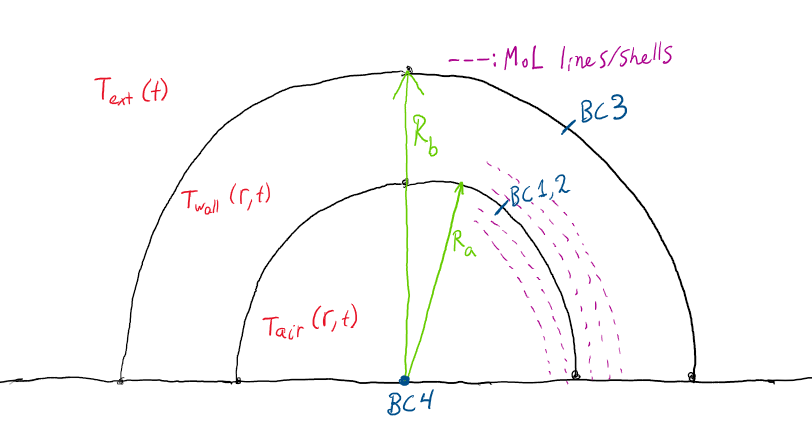
\includegraphics[width=0.5\linewidth]{Model Diagram.PNG}
    \caption{Rough Sketch of the Hut}
    \label{Model Sketch}
\end{figure}

\subsection{Plots}

\begin{figure}[h]
    \centering
    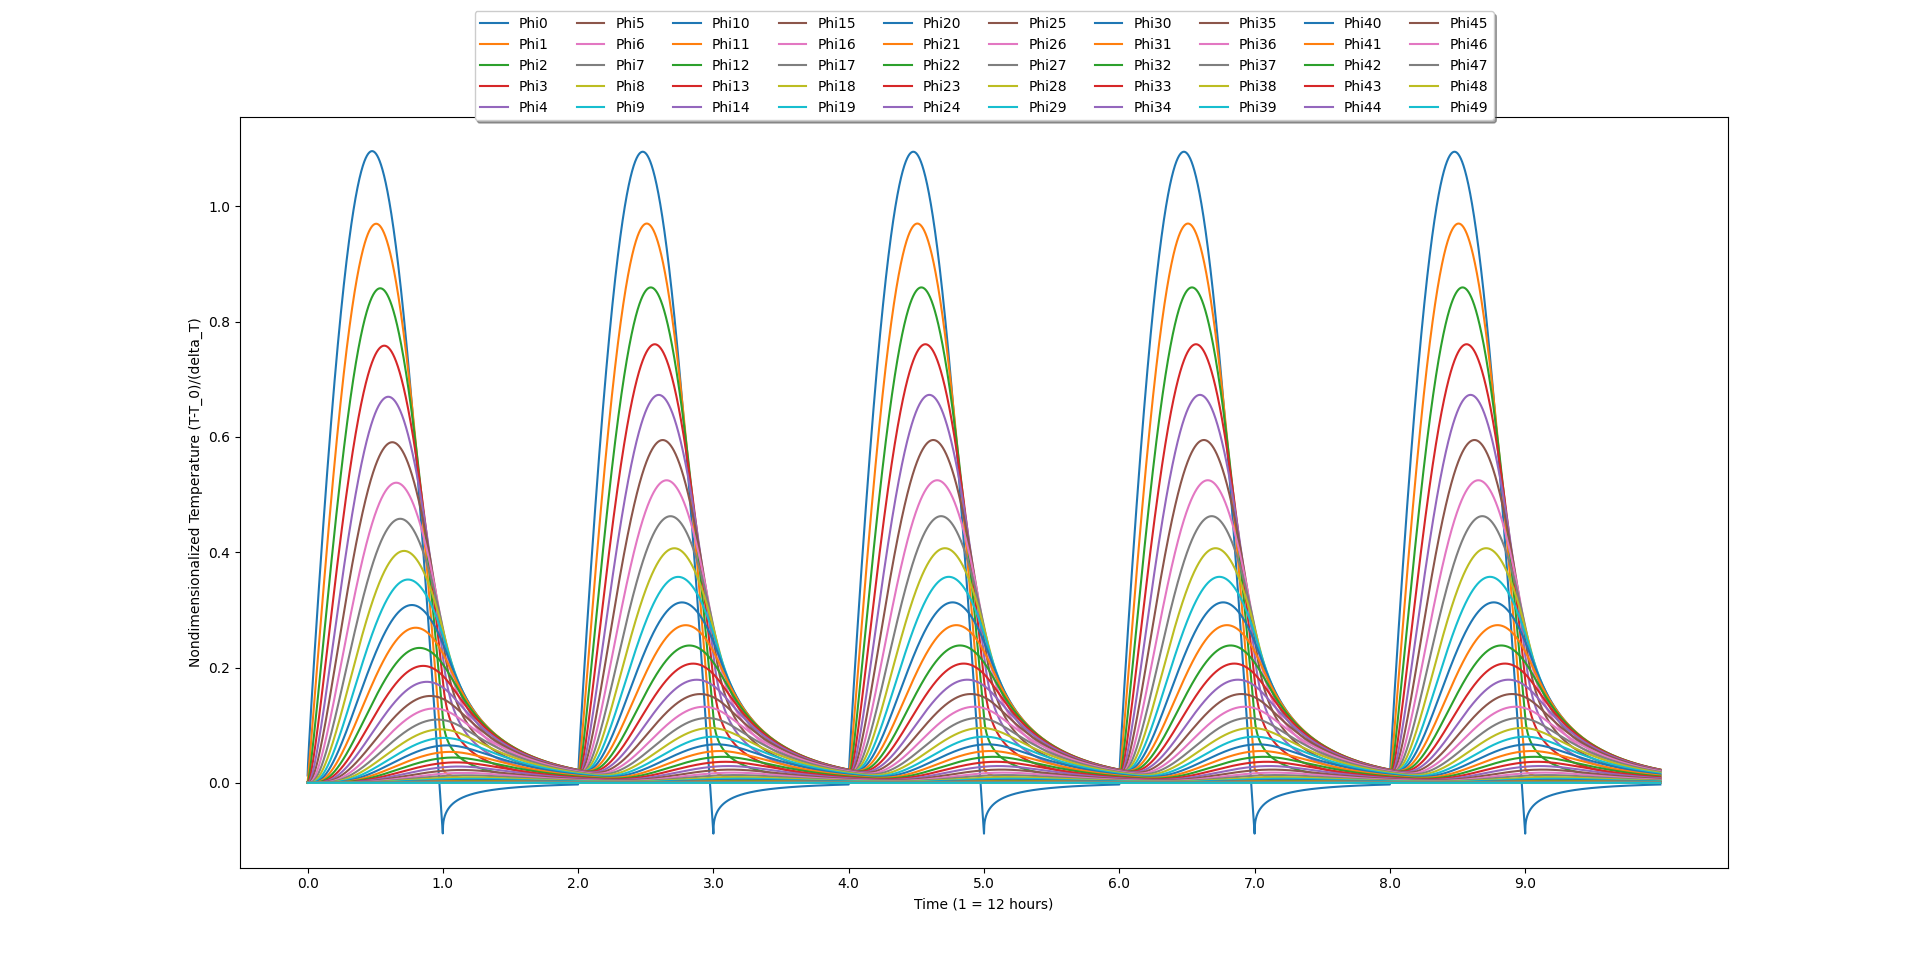
\includegraphics[width=0.8\linewidth]{2D Plot.png}
    \caption{2D Plot of temperature in each shell vs. Time}
    \label{2d plot}
\end{figure}

\pagebreak
\begin{figure}[h]
    \centering
    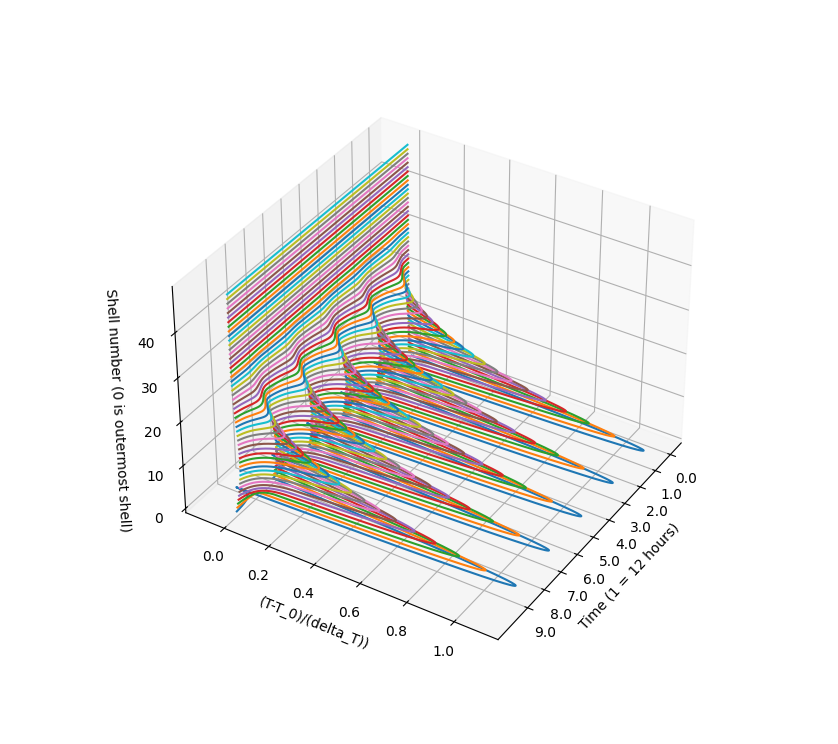
\includegraphics[width=0.8\linewidth]{3D Plot.png}
    \caption{3D Plot of temperature in each shell vs. Time}
    \label{3d plot}
\end{figure}

\end{document}